%!TEX encoding = UTF-8 Unicode
% Author: Laurent Dutriaux
\documentclass[a4paper,11pt,landscape]{article}
\usepackage{geometry}
 \geometry{
 a4paper,
 total={257mm,170mm},
 left=10mm,
 top=10mm,
 }
\usepackage[utf8]{inputenc}
\usepackage{fourier} % Utilisation des polices texte
\usepackage{tikz}
\usetikzlibrary[positioning]
\usetikzlibrary{patterns}
%\usepackage[french]{babel} % styles français
\title{Timeplan 3AUA}
\newcommand{\daywidth}{4.5 cm}
\begin{document}

\maketitle

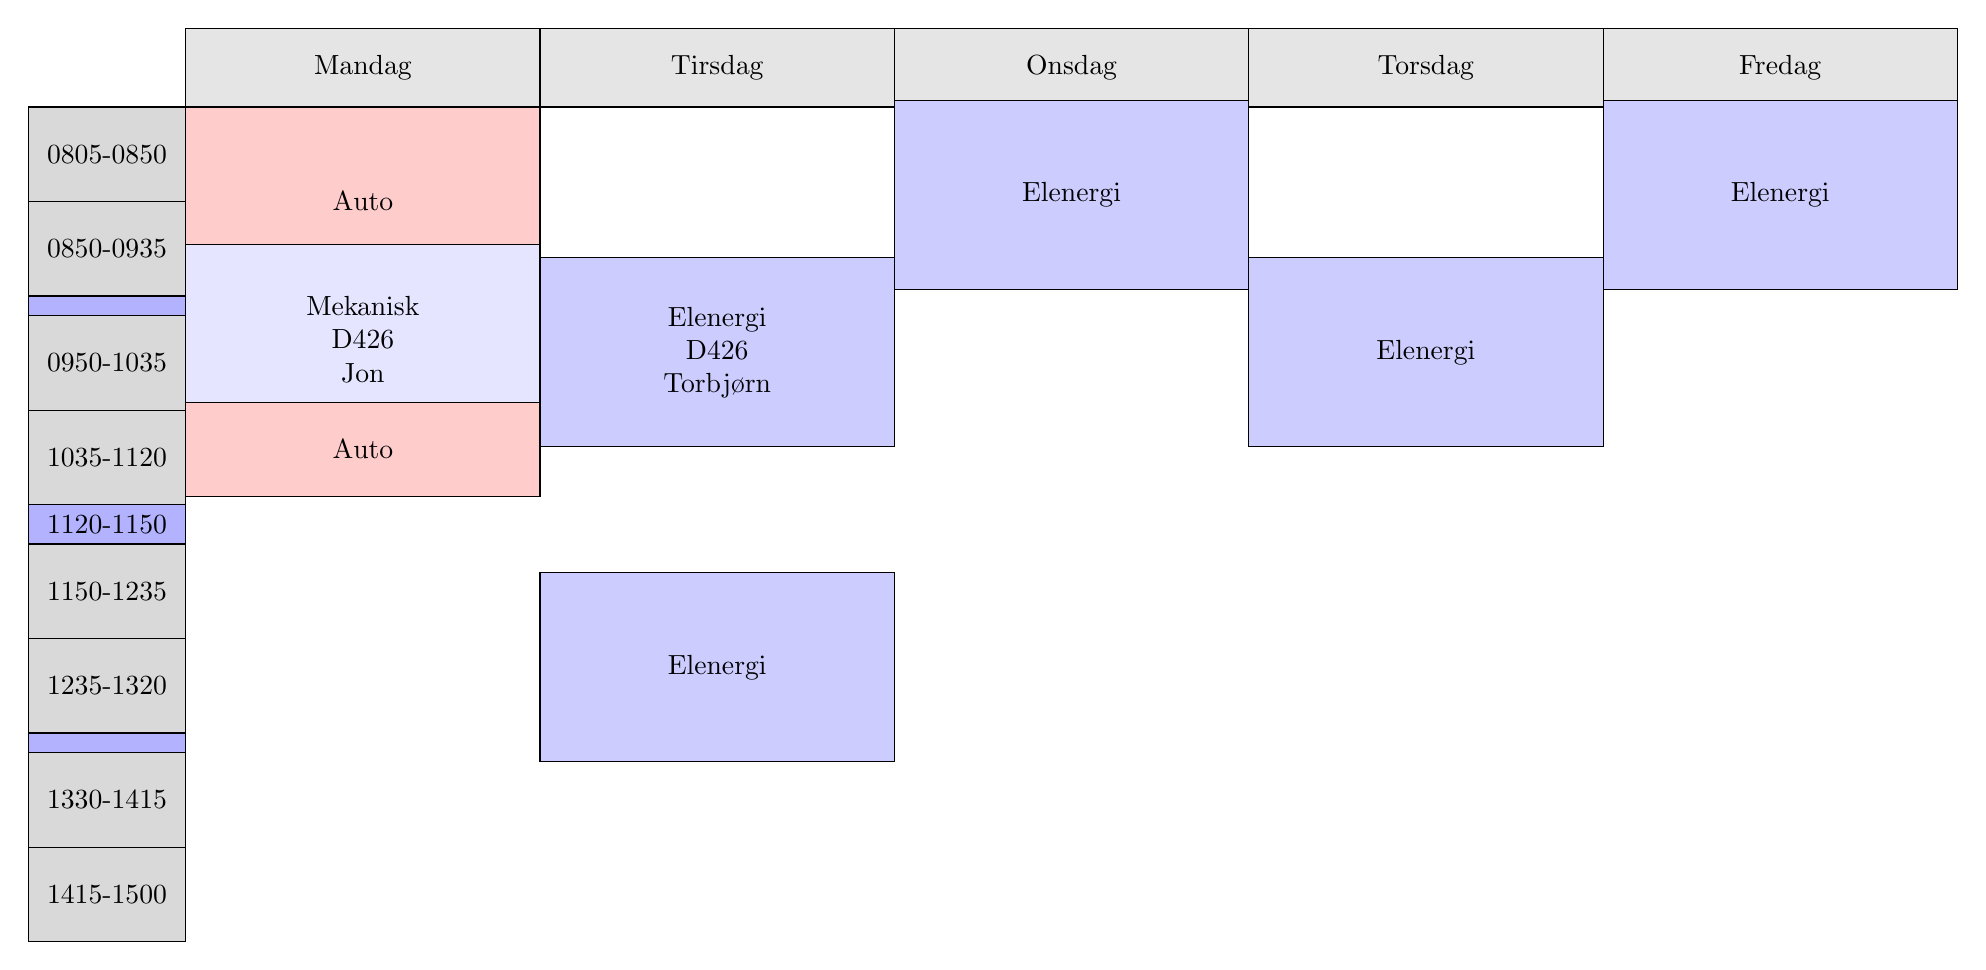
\begin{tikzpicture}[x=\daywidth, y=-1cm, node distance=0 cm,outer sep = 0pt]
% Style for Days
\tikzstyle{day}=[draw, rectangle,  minimum height=1cm, minimum width=\daywidth, fill=gray!20,anchor=south west]
% Style for hours
\tikzstyle{hour}=[draw, rectangle, minimum height=1.2 cm, minimum width=2 cm, fill=gray!30,anchor=north east]
\tikzstyle{friminutt}=[draw, rectangle, minimum height=0.25 cm, minimum width=2 cm, fill=blue!30,anchor=north east]
\tikzstyle{mat}=[draw, rectangle, minimum height=0.5 cm, minimum width=2 cm, fill=blue!30,anchor=north east]

% Styles for events
% Duration of sequences
\tikzstyle{hours}=[rectangle,draw, minimum width=\daywidth, anchor=north west,text centered,text width=5 em]
\tikzstyle{1hour}=[hours,minimum height=1.2cm]
\tikzstyle{2hours}=[hours,minimum height=2.4cm]
\tikzstyle{3hours}=[hours,minimum height=3.6cm]
%Style for type of sequence 
\tikzstyle{Auto1h}=[1hour,fill=red!20]
\tikzstyle{Auto2h}=[2hours,fill=red!20]
\tikzstyle{Elenergi1h}=[1hour,fill=blue!20]
\tikzstyle{Elenergi2h}=[2hours,fill=blue!20]
\tikzstyle{Mek1h}=[1hour,fill=blue!10]
\tikzstyle{Mek2h}=[2hours,fill=blue!10]
\tikzstyle{TP2h}=[2hours, pattern=north east lines, pattern color=magenta]
\tikzstyle{G3h}=[3hours, pattern=north west lines, pattern color=magenta!60!white]
\tikzstyle{Planche}=[1hour,fill=white]
% Positioning labels for days and hours
\node[day] (man) at (1,8.083333) {Mandag};
\node[day] (tir) [right = of man] {Tirsdag};
\node[day] (ons) [right = of tir] {Onsdag};
\node[day] (tor) [right = of ons] {Torsdag};
\node[day] (fre) [right = of tor] {Fredag};
\node[hour] (1) at (1,8.083333) {0805-0850};
\node[hour] (2) [below = of 1] {0850-0935};
\node[friminutt] (fr1) [below = of 2] {};
\node[hour] (3) [below= of fr1] {0950-1035};
\node[hour] (4) [below = of 3] {1035-1120};
\node[mat] (mat) [below = of 4] {1120-1150};
\node[hour] (5) [below = of mat] {1150-1235};
\node[hour] (6) [below = of 5] {1235-1320};
\node[friminutt] (fr1) [below = of 6] {};
\node[hour] (7) [below = of fr1] {1330-1415};
\node[hour] (8) [below = of 7] {1415-1500};
%Position of sequences
\node[Auto2h] at (1,8.083333) {Auto};
\node[Mek2h] at (1,9.83333) {Mekanisk\\D426\\Jon};
\node[Auto1h] at (1,11.83333) {Auto};
\node[Elenergi2h] at (2,10) {Elenergi\\D426\\Torbjørn};
\node[Elenergi2h] at (2,14) {Elenergi};
\node[Elenergi2h] at (3,8) {Elenergi};
\node[Elenergi2h] at (4,10) {Elenergi};
\node[Elenergi2h] at (5,8) {Elenergi};
\end{tikzpicture}


\end{document} 
